% Generated by ArticleSignalDiagrams. Opaque vector fills only.
\documentclass[10pt,tikz,border=5pt]{standalone}
\usepackage{lmodern}
\usetikzlibrary{fit}
\begin{document}
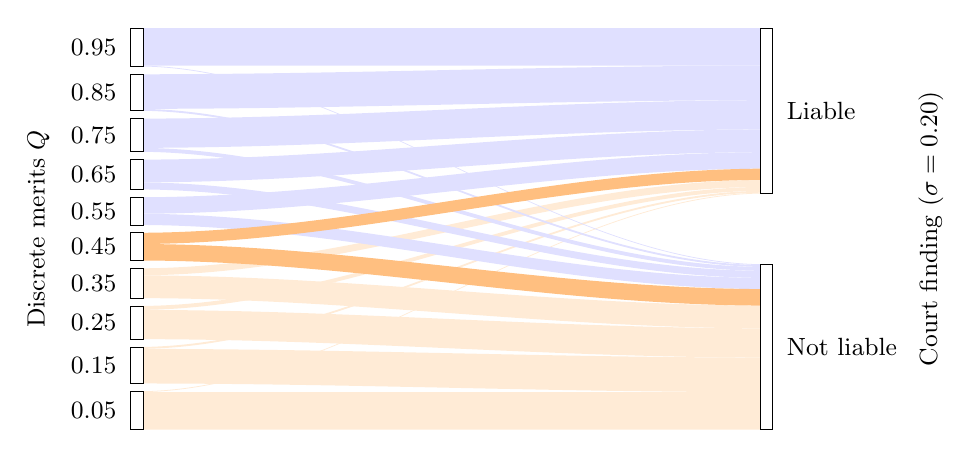
\begin{tikzpicture}[x=1cm,y=1cm,font=\small]\path[fill=orange!16!white,draw=none] (3.3,-5.1) .. controls (6,-5.1) and (8.6,-5.1) .. (11.3,-5.1) -- (11.3,-4.623268) .. controls (8.6,-4.623268) and (6,-4.623268) .. (3.3,-4.623268) -- cycle;
\path[fill=orange!16!white,draw=none] (3.3,-4.623268) .. controls (6,-4.623268) and (8.6,-2.1) .. (11.3,-2.1) -- (11.3,-2.090064) .. controls (8.6,-2.090064) and (6,-4.613332) .. (3.3,-4.613332) -- cycle;
\path[fill=orange!16!white,draw=none] (3.3,-4.513332) .. controls (6,-4.513332) and (8.6,-4.623268) .. (11.3,-4.623268) -- (11.3,-4.18425) .. controls (8.6,-4.18425) and (6,-4.074314) .. (3.3,-4.074314) -- cycle;
\path[fill=orange!16!white,draw=none] (3.3,-4.074314) .. controls (6,-4.074314) and (8.6,-2.090064) .. (11.3,-2.090064) -- (11.3,-2.066088) .. controls (8.6,-2.066088) and (6,-4.050338) .. (3.3,-4.050338) -- cycle;
\path[fill=orange!16!white,draw=none] (3.3,-3.950338) .. controls (6,-3.950338) and (8.6,-4.18425) .. (11.3,-4.18425) -- (11.3,-3.813033) .. controls (8.6,-3.813033) and (6,-3.579121) .. (3.3,-3.579121) -- cycle;
\path[fill=orange!16!white,draw=none] (3.3,-3.579121) .. controls (6,-3.579121) and (8.6,-2.066088) .. (11.3,-2.066088) -- (11.3,-2.016403) .. controls (8.6,-2.016403) and (6,-3.529436) .. (3.3,-3.529436) -- cycle;
\path[fill=orange!16!white,draw=none] (3.3,-3.429436) .. controls (6,-3.429436) and (8.6,-3.813033) .. (11.3,-3.813033) -- (11.3,-3.524078) .. controls (8.6,-3.524078) and (6,-3.140481) .. (3.3,-3.140481) -- cycle;
\path[fill=orange!16!white,draw=none] (3.3,-3.140481) .. controls (6,-3.140481) and (8.6,-2.016403) .. (11.3,-2.016403) -- (11.3,-1.92733) .. controls (8.6,-1.92733) and (6,-3.051408) .. (3.3,-3.051408) -- cycle;
\path[fill=blue!12!white,draw=none] (3.3,-2.5) .. controls (6,-2.5) and (8.6,-3.314801) .. (11.3,-3.314801) -- (11.3,-3.17267) .. controls (8.6,-3.17267) and (6,-2.357868) .. (3.3,-2.357868) -- cycle;
\path[fill=blue!12!white,draw=none] (3.3,-2.357868) .. controls (6,-2.357868) and (8.6,-1.785199) .. (11.3,-1.785199) -- (11.3,-1.575922) .. controls (8.6,-1.575922) and (6,-2.148592) .. (3.3,-2.148592) -- cycle;
\path[fill=blue!12!white,draw=none] (3.3,-2.048592) .. controls (6,-2.048592) and (8.6,-3.17267) .. (11.3,-3.17267) -- (11.3,-3.083597) .. controls (8.6,-3.083597) and (6,-1.959519) .. (3.3,-1.959519) -- cycle;
\path[fill=blue!12!white,draw=none] (3.3,-1.959519) .. controls (6,-1.959519) and (8.6,-1.575922) .. (11.3,-1.575922) -- (11.3,-1.286967) .. controls (8.6,-1.286967) and (6,-1.670564) .. (3.3,-1.670564) -- cycle;
\path[fill=blue!12!white,draw=none] (3.3,-1.570564) .. controls (6,-1.570564) and (8.6,-3.083597) .. (11.3,-3.083597) -- (11.3,-3.033912) .. controls (8.6,-3.033912) and (6,-1.520879) .. (3.3,-1.520879) -- cycle;
\path[fill=blue!12!white,draw=none] (3.3,-1.520879) .. controls (6,-1.520879) and (8.6,-1.286967) .. (11.3,-1.286967) -- (11.3,-0.91575) .. controls (8.6,-0.91575) and (6,-1.149662) .. (3.3,-1.149662) -- cycle;
\path[fill=blue!12!white,draw=none] (3.3,-1.049662) .. controls (6,-1.049662) and (8.6,-3.033912) .. (11.3,-3.033912) -- (11.3,-3.009936) .. controls (8.6,-3.009936) and (6,-1.025686) .. (3.3,-1.025686) -- cycle;
\path[fill=blue!12!white,draw=none] (3.3,-1.025686) .. controls (6,-1.025686) and (8.6,-0.91575) .. (11.3,-0.91575) -- (11.3,-0.476732) .. controls (8.6,-0.476732) and (6,-0.586668) .. (3.3,-0.586668) -- cycle;
\path[fill=blue!12!white,draw=none] (3.3,-0.486668) .. controls (6,-0.486668) and (8.6,-3.009936) .. (11.3,-3.009936) -- (11.3,-3) .. controls (8.6,-3) and (6,-0.476732) .. (3.3,-0.476732) -- cycle;
\path[fill=blue!12!white,draw=none] (3.3,-0.476732) .. controls (6,-0.476732) and (8.6,-0.476732) .. (11.3,-0.476732) -- (11.3,0) .. controls (8.6,0) and (6,-0) .. (3.3,-0) -- cycle;
\path[fill=orange!50!white,draw=none] (3.3,-2.951408) .. controls (6,-2.951408) and (8.6,-3.524078) .. (11.3,-3.524078) -- (11.3,-3.314801) .. controls (8.6,-3.314801) and (6,-2.742132) .. (3.3,-2.742132) -- cycle;
\path[fill=orange!50!white,draw=none] (3.3,-2.742132) .. controls (6,-2.742132) and (8.6,-1.92733) .. (11.3,-1.92733) -- (11.3,-1.785199) .. controls (8.6,-1.785199) and (6,-2.6) .. (3.3,-2.6) -- cycle;
\coordinate (axis-midline-0) at (0,-2.55);
\path[fill=white,draw=black,line width=0.3pt] (3.22,-5.1) rectangle (3.38,-4.613332);
\node[anchor=east,fill=white,inner sep=2pt] (bucket-0-0-0) at (3.12,-4.856666) {0.05};
\path[fill=white,draw=black,line width=0.3pt] (3.22,-4.513332) rectangle (3.38,-4.050338);
\node[anchor=east,fill=white,inner sep=2pt] (bucket-0-0-1) at (3.12,-4.281835) {0.15};
\path[fill=white,draw=black,line width=0.3pt] (3.22,-3.950338) rectangle (3.38,-3.529436);
\node[anchor=east,fill=white,inner sep=2pt] (bucket-0-0-2) at (3.12,-3.739887) {0.25};
\path[fill=white,draw=black,line width=0.3pt] (3.22,-3.429436) rectangle (3.38,-3.051408);
\node[anchor=east,fill=white,inner sep=2pt] (bucket-0-0-3) at (3.12,-3.240422) {0.35};
\path[fill=white,draw=black,line width=0.3pt] (3.22,-2.951408) rectangle (3.38,-2.6);
\node[anchor=east,fill=white,inner sep=2pt] (bucket-0-0-4) at (3.12,-2.775704) {0.45};
\path[fill=white,draw=black,line width=0.3pt] (3.22,-2.5) rectangle (3.38,-2.148592);
\node[anchor=east,fill=white,inner sep=2pt] (bucket-0-0-5) at (3.12,-2.324296) {0.55};
\path[fill=white,draw=black,line width=0.3pt] (3.22,-2.048592) rectangle (3.38,-1.670564);
\node[anchor=east,fill=white,inner sep=2pt] (bucket-0-0-6) at (3.12,-1.859578) {0.65};
\path[fill=white,draw=black,line width=0.3pt] (3.22,-1.570564) rectangle (3.38,-1.149662);
\node[anchor=east,fill=white,inner sep=2pt] (bucket-0-0-7) at (3.12,-1.360113) {0.75};
\path[fill=white,draw=black,line width=0.3pt] (3.22,-1.049662) rectangle (3.38,-0.586668);
\node[anchor=east,fill=white,inner sep=2pt] (bucket-0-0-8) at (3.12,-0.818165) {0.85};
\path[fill=white,draw=black,line width=0.3pt] (3.22,-0.486668) rectangle (3.38,-0);
\node[anchor=east,fill=white,inner sep=2pt] (bucket-0-0-9) at (3.12,-0.243334) {0.95};
\node[fit=(bucket-0-0-0) (bucket-0-0-1) (bucket-0-0-2) (bucket-0-0-3) (bucket-0-0-4) (bucket-0-0-5) (bucket-0-0-6) (bucket-0-0-7) (bucket-0-0-8) (bucket-0-0-9),inner sep=0pt] (source-labels-0) {};
\coordinate (axis-title-0-0) at (source-labels-0.west |- axis-midline-0);
\node[rotate=90,anchor=south,inner sep=0pt] at ([xshift=-0.18cm]axis-title-0-0) {Discrete merits $Q$};
\path[fill=white,draw=black,line width=0.3pt] (11.22,-5.1) rectangle (11.38,-3);
\node[anchor=west,fill=white,inner sep=2pt] (bucket-0-1-0) at (11.48,-4.05) {Not liable};
\path[fill=white,draw=black,line width=0.3pt] (11.22,-2.1) rectangle (11.38,0);
\node[anchor=west,fill=white,inner sep=2pt] (bucket-0-1-1) at (11.48,-1.05) {Liable};
\node[fit=(bucket-0-1-0) (bucket-0-1-1),inner sep=0pt] (destination-labels-0) {};
\coordinate (axis-title-0-1) at (destination-labels-0.east |- axis-midline-0);
\node[rotate=90,anchor=north,inner sep=0pt] at ([xshift=0.18cm]axis-title-0-1) {Court finding ($\sigma=0.20$)};
\end{tikzpicture}
\end{document}

